\subsection{Research}

Ein Research Honeypot wird für die Untersuchung und Forschung der Angriffe eingesetzt. Der Honeypot wird meist getrennt von allen Produktivsystemen aufgebaut. In Abbildung 1.1 wird der Honeypot vor die Firewall des Produktivnetzes installiert. Dadurch wird versucht mögliche Angreifer weit weg von dem Produktiv-Systemen zu halten. 
\\
\begin{figure}[ht]
    \centering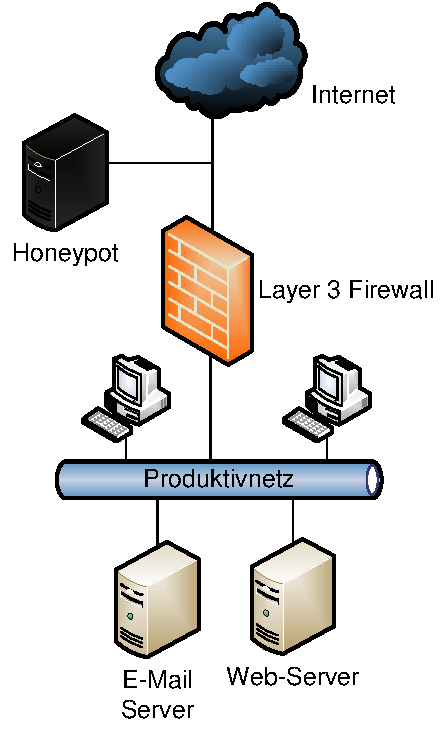
\includegraphics[scale=0.6]{Bilder/Research_1.pdf}
  \caption{Research Honeypot}
  \label{hnet:geni}
\end{figure}


Eine weitere Möglichkeit eines solchen Aufbaus ist in Abbildung 1.2 dargestellt. Hier wird der Honeypot durch die Layer 3 Firewall von dem Produktivnetz getrennt. Bei diesem Aufbau muss genau auf die Firewall-Einstellungen geachtet werden, um den Angreifern nicht ungewollt einen Sprungserver zu den produktiven Systemen zur Verfügung zu stellen.
\\
\begin{figure}[ht]
    \centering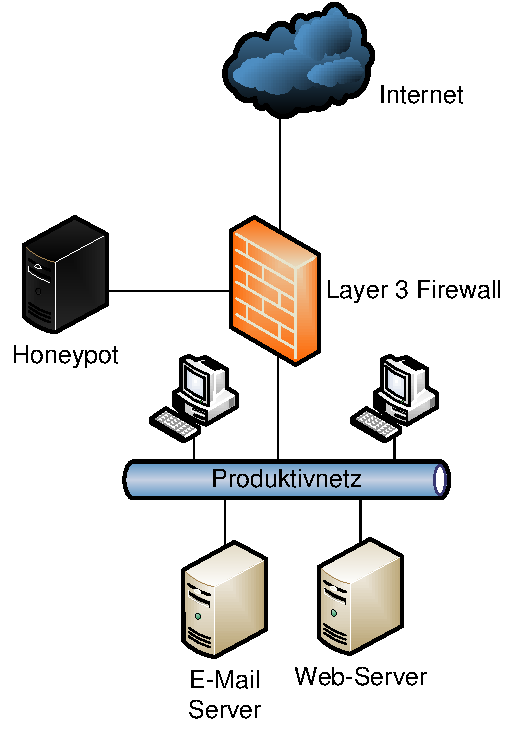
\includegraphics[scale=0.6]{Bilder/Research_2.pdf}
  \caption{Research Honeypot}
  \label{hnet:geni}
\end{figure}

Es geht hier primär um die Erkennung von neuen Würmern, Trojanern und weiterer Schadsoftware. Neben der Schadsoftware werden auch Angriffe von Hackern sowie der nicht so qualifizierten \glqq Skript-Kiddies\grqq untersucht.

Bei jedem Angriff werden Daten und Informationen über den Angreifer gesammelt. Dabei lässt sich häufig ermitteln wer, womit und evtl. auch warum er angegriffen hat. Setzt man mehrere Honeypots an verschiedenen Standorten ein, lassen sich mit den gesammelten Daten neue Trends der Angreifer erkennen. Durch diese Informationen versuchen Unternehmen Angriffe auch vorhersagen zu können und die Vorgehensweise der Angreifer besser zu verstehen. Mit den gesammelten Daten können auch neue Tools, mit denen vorallem Skript-Kiddies arbeiten, aufgedeckt werden.

Um die Daten besser auswerten zu können teilen verschiedene Organisationen ihre gesammelten Daten und Erkenntnisse mit anderen Unternehmen. Die große Anzahl der Daten ermöglicht eine bessere Analyse sowie eine genauere Trend-Erkennung. 

Research Honeypots dienen somit nicht direkt zur Risiko-Minimierung. Vielmehr helfen die Erkenntnisse, die Angriffs-Prävention und Erkennung zu verbessern.